\documentclass[11pt,a4paper]{article}
\usepackage{{../../paquete-formulas}}
\usepackage{{../../estilos-formulas}}


\newcommand{\materia}{Mecánica de Fluidos y Máquinas Fluidodinámicas}

%Comando para variables y sus unidades
\newcommand{\variable}[2]{$#1$ $\left[#2\right]$}
%Comando para grados
\newcommand{\grado}{^\circ}
%Comando para el volumen desplazado
\newcommand{\vdes}{\st{\textsl{V}}}

\begin{document}
	\pagestyle{pieyencabezado}
	\section*{Nomenclatura}
	
		\begin{center}
			\begin{tabular}{r l r l}
			\variable{V}{m^3} & Volumen & \variable{W}{kgf} & Peso\\
			\variable{\mu}{Pa \cdot s} & Viscosidad absoluta & \variable{v}{m^2/s} & Viscosidad cinemática\\
			\variable{\sigma}{N/m} & Tensión superficial & $\overline{GM}$ & Altura metacéntrica\\
			$G$ & Centro de gravedad & $C$ & Centro de presión\\
			\variable{\rho}{kg/m^3} & Densidad & $\rho_{rel}$ & Densidad relativa\\
			\variable{\tau}{N/m^2} & Esfuerzo de corte & $g=9.8 \sfrac{m}{s^2}$ & Aceleración de la gravedad\\
			\variable{W}{kgf}& Peso & \variable{\gamma}{kgf/m^3}& Peso específico\\
			\variable{J}{m^4} & Segundo momento & \variable{\overline{J}}{m^4} & Segundo momento respecto a G\\
		\end{tabular}
		\end{center}
	\section*{Conversión de unidades}
		\begin{tabular}{r l r l}
			Presión & & & \\
			Temperatura & $K =\ \grado C + 273.15$ & $ \grado R\ =\ \grado F + 459.67$ & \\
		\end{tabular}
	\unidad{1}{Conceptos generales}
	\begin{multicols}{2}
		\begin{cajita}
				\subtitulo{Presión \vspace{.085cm}}
				\begin{tabular}{l l}
					\multicolumn{2}{c}{$P_{absoluta} = P_{atmosférica} + P_{manométrica}$\vspace{.1cm}}\\
					$P_{man} (+)$ & Presión manométrica\vspace{.1cm} \\
					$P_{man} (-)$ & Vacío \\
				\end{tabular}
				\columnbreak
		\end{cajita}
		\begin{cajita}		
				\subtitulo{Densidad y peso específico}
				$\rho_{rel} = \dfrac{\rho}{\rho_{H_2O}}$\vspace{.1cm}\\
				$\gamma = \dfrac{W}{V} = \dfrac{mg}{V} = \rho g$\\
		\end{cajita}
	\end{multicols}
	\begin{multicols}{2}
		\begin{cajita}		
				\subtitulo{Viscosidad\vspace{.08cm}}
				\begin{tabular}{l l}
					$\tau = \mu \dfrac{du}{dy}$ & $v = \dfrac{\mu}{\delta}$\\
					Fluido newtoniano & $\mu = cte$ \\
					Fluido ideal & $\mu = 0$
				\end{tabular}
			
		\end{cajita}
		\begin{cajita}
			
				\subtitulo{Tensión superficial}
				\begin{tabular}{l l}
					No sé que pingo poner acá & help...\\
					Capilaridad & $h = \dfrac{4 \sigma \cos \beta}{\gamma D}$
				\end{tabular}
		
		También pensaba poner la ecuación de los gases y algo de ese estilo que vimos en termo... pero no sé, qué opinan ustedes?
			
		\end{cajita}
	\end{multicols}
	
	\unidad{2}{Estática de los fluidos}
	
	\begin{multicols}{2}
		\begin{cajita}
			\subtitulo{Fluidos en reposo}\vspace{.1cm}
			
			$dp = -\gamma dz$
			
			
		\end{cajita}
	
		\begin{cajita}
			\subtitulo{Fuerzas sobre áreas planas}\vspace{.1cm}
			
			\begin{tabular}{l l}
				Magnitud de F & $F = \gamma \bar{h} A$\\ & \hspace{.2cm} $= P_C A$\\
				Punto de aplicación de F & $ y_P = \bar{y} + \dfrac{\bar{J}}{A \bar{y}}$\\
				$C:(x_P, y_P)$& $x_P = \bar{x} + \dfrac{\bar{J}_{xy}}{A \bar{y}}$\\
			\end{tabular}
		\end{cajita}
	
		\begin{cajita}
			\subtitulo{Flotabilidad}\vspace{.1cm}
			
			\begin{tabular}{l l}
				\multicolumn{2}{c}{$F_B = \gamma \vdes$}\\
				En equilibrio & $F=W$\\
			\end{tabular}
		
		\end{cajita}
	
		\begin{cajita}
			\subtitulo{Estabilidad}\vspace{.1cm}
			
			Altura metacéntrica\\
			$\overline{GM} = \dfrac{J_O}{\vdes} - \overline{CG}$\\
			Momento restaurador\\
			$C=\gamma_{fluido}~\Delta \theta_{radianes}~J_O$ 
			
			
%			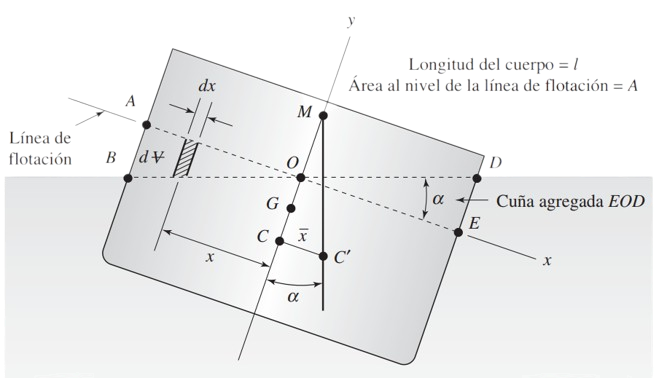
\includegraphics[width=\linewidth]{estabilidad}
			
		\end{cajita}
		
		\begin{cajita}
			\subtitulo{Recipientes linealmente acelerados}\vspace{.1cm}
			
			
			$dp=-\rho a_x dx~-~\rho(g +a_z)dz$\\
			En la misma linea de presión $(p_1 = p_2)$\\
			$\dfrac{z_1-z_2}{x_2-x_1}=tan(\alpha)=\dfrac{a_x}{g+a_z}$
			
			
			%			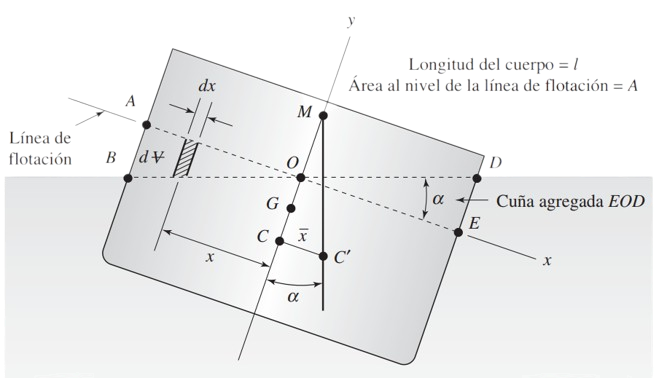
\includegraphics[width=\linewidth]{estabilidad}
			
		\end{cajita}
		
		\begin{cajita}
			\subtitulo{Flujo}\vspace{.1cm}
			
			Bernoulli\\
			$\dfrac{p_1}{\gamma}+\dfrac{v_1^2}{2g}+z_1=\dfrac{p_2}{\gamma}+\dfrac{v_2^2}{2g}+z_2$\\
			Flujo con perdidas, bomba y turbina\\
			$H_p+\dfrac{p_1}{\gamma}+\dfrac{v_1^2}{2g}+z_1=H_T+\dfrac{p_2}{\gamma}+\dfrac{v_2^2}{2g}+z_2+h_L$\\
			Perdidas:\\
			$h_L= K\dfrac{v^2}{2g}$\\
			
			
			\textbf{FLUJO INTERNO(?}
			Nro de Reynols $Re=\dfrac{V~D}{\nu}$\\
			Perdida de carga $h_L=\dfrac{\Delta p}{\gamma}=f~\dfrac{L}{D}\dfrac{v^2}{2g}$\\
			para flujo laminar en un tubo $f=64/Re$\\
			Para otros flujos Moody o las ecuaciones
			\vspace*{0.5cm}
			
\textbf{Perdidas en conductos no circulares}\\
			Radio hidráulico $R_H=\dfrac{Sección~transversal }{preimetro~mojado}$\\
			con: $Re=\dfrac{4RV}{\nu}$ y rugosidad relativa $=\dfrac{e}{4R}$\\
			Queda $hL=f~\dfrac{L}{4R}\dfrac{v^2}{2g}$\\
	\textbf{Otras formas de calcular perdidas}\\
	$L_{eq}=K\frac{D}{f}$\\
	Perdidas con Hazen-William \\
	$K=\dfrac{10.68~Q^{1.85}}{C^{1.85}D^{4.85}}$\\
	$Hf=L_{eq}*K$\\
	
	\textbf{Flujo turbulento}\\
	$h_L=1.07\dfrac{Q^2L}{gD^5}\left\{ln\left[ \dfrac{e}{3.7D}+4.62 \left(\dfrac{\nu D}{Q}\right)^{0.9} \right]\right\}^{-2}$\\
	Eso aplica para\\ $10^{-6}<e/D<10^{-2}$ y $3000<Re<3x10^8$\\ \vspace*{0.25cm}
	
	$Q=-0.965\left(\dfrac{gD^5h_L}{L}\right)^{0.5}ln\left[\dfrac{e}{3.7D}+\left(\dfrac{3.17\nu^2L}{gD^3h_L}\right)^{0.5}\right]$\\
	Esto aplica para $Re>2000$\\ \vspace*{0.25cm}
	
	$D=0.66\left[e^{1.25}\left(\dfrac{LQ^2}{gh_L}\right)^{4.75}+\nu Q^{9.4}\left(\dfrac{L}{gh_L}^{5.2}\right)\right]^{0.04}$\\
	Esto aplica para:\\$10^{-6}<e/D<10^{-2}$ y $5000<Re<3x10^8$\\ \vspace*{0.25cm}
		\end{cajita}
		
		
		\begin{cajita}
			\subtitulo{Cierre}\vspace{.1cm}
			Celeridad $a=\dfrac{\sqrt{\frac{K}{\rho}}}{\sqrt{1+\psi \frac{K}{E} \frac{D}{e}}}$, $(\psi\rightarrow1)$
			Pulso Joukowsky\\ \vspace{.1cm}
			Cierre instantaneo:$\Delta H=\dfrac{a V_0}{g}$\\\vspace{.1cm}
			Cierre lento: $\Delta H_m=\dfrac{2 L V_0}{g~T_c}$\\\vspace{.1cm}
			Tiempo crítico: $Tc=2L/a$\\
		\end{cajita}

	\begin{cajita}
		Expresiones de perdidas y Reynols en caudala\\
		$Re=\dfrac{4Q}{\pi D \nu}$\\
		$H_f=\dfrac{16 f l Q^{2}}{2 g \pi^{2} D^{5}}$
		
	\end{cajita}
		
	\end{multicols}	
			
			
\end{document}